The stability of the ten photodiodes used to survey the \laser~light is monitored with a LED signal. The light is also transmitted to a reference photodiode for normalization. This reference photodiode is itself monitor thanks to a radioactive source.\\
A view of the PHOCAL box is given on figure \ref{fig:lasphocal}. It is comprised of:
\begin{itemize}
\item LED box: houses the LED (Nichia blue NSPB520S $\lambda$=520 nm) itself and an LED driver that provides a pulsed signal lasting 10 ns with an intensity that may be tweaked manually thanks to a potentiometer between 20 and 20 V.
\item reference box: the reference photodiode is located in this box. It receives the LED signal through an optics fiber connected to the LED box. The stability of this photodiode is monitored thanks to a radioactive $\alpha$-source of $^{241}$Am (T$_{1/2}$=432.2 y, E_${\alpha}$=5.486 MeV) placed in front of it. Because of their charge and large mass, alpha particles can travel only a few centimetres in air. To maximize the radioactive signal dry air is injected on the reference photodiode.
\item Logic board: this card is used to drive the PHOCAL system. It provides a 90 Hz signal to trigger the LED signal. This frequency has been chosen so as to keep the coïncidence rate of the radioactive source and the LED signals at the sub-percent level.
\item optics fibers and light mixers: the LED signal is transmitted to optics fibers through PMMA pieces (square section: ; length:) 
\end{itemize}
Two temperature (one in the reference box, the other in the LED box) and one humidity (in the reference box) probes are used to measure the environmental conditions in the PHOCAL box. 

\begin{figure}[htbp]
\centering
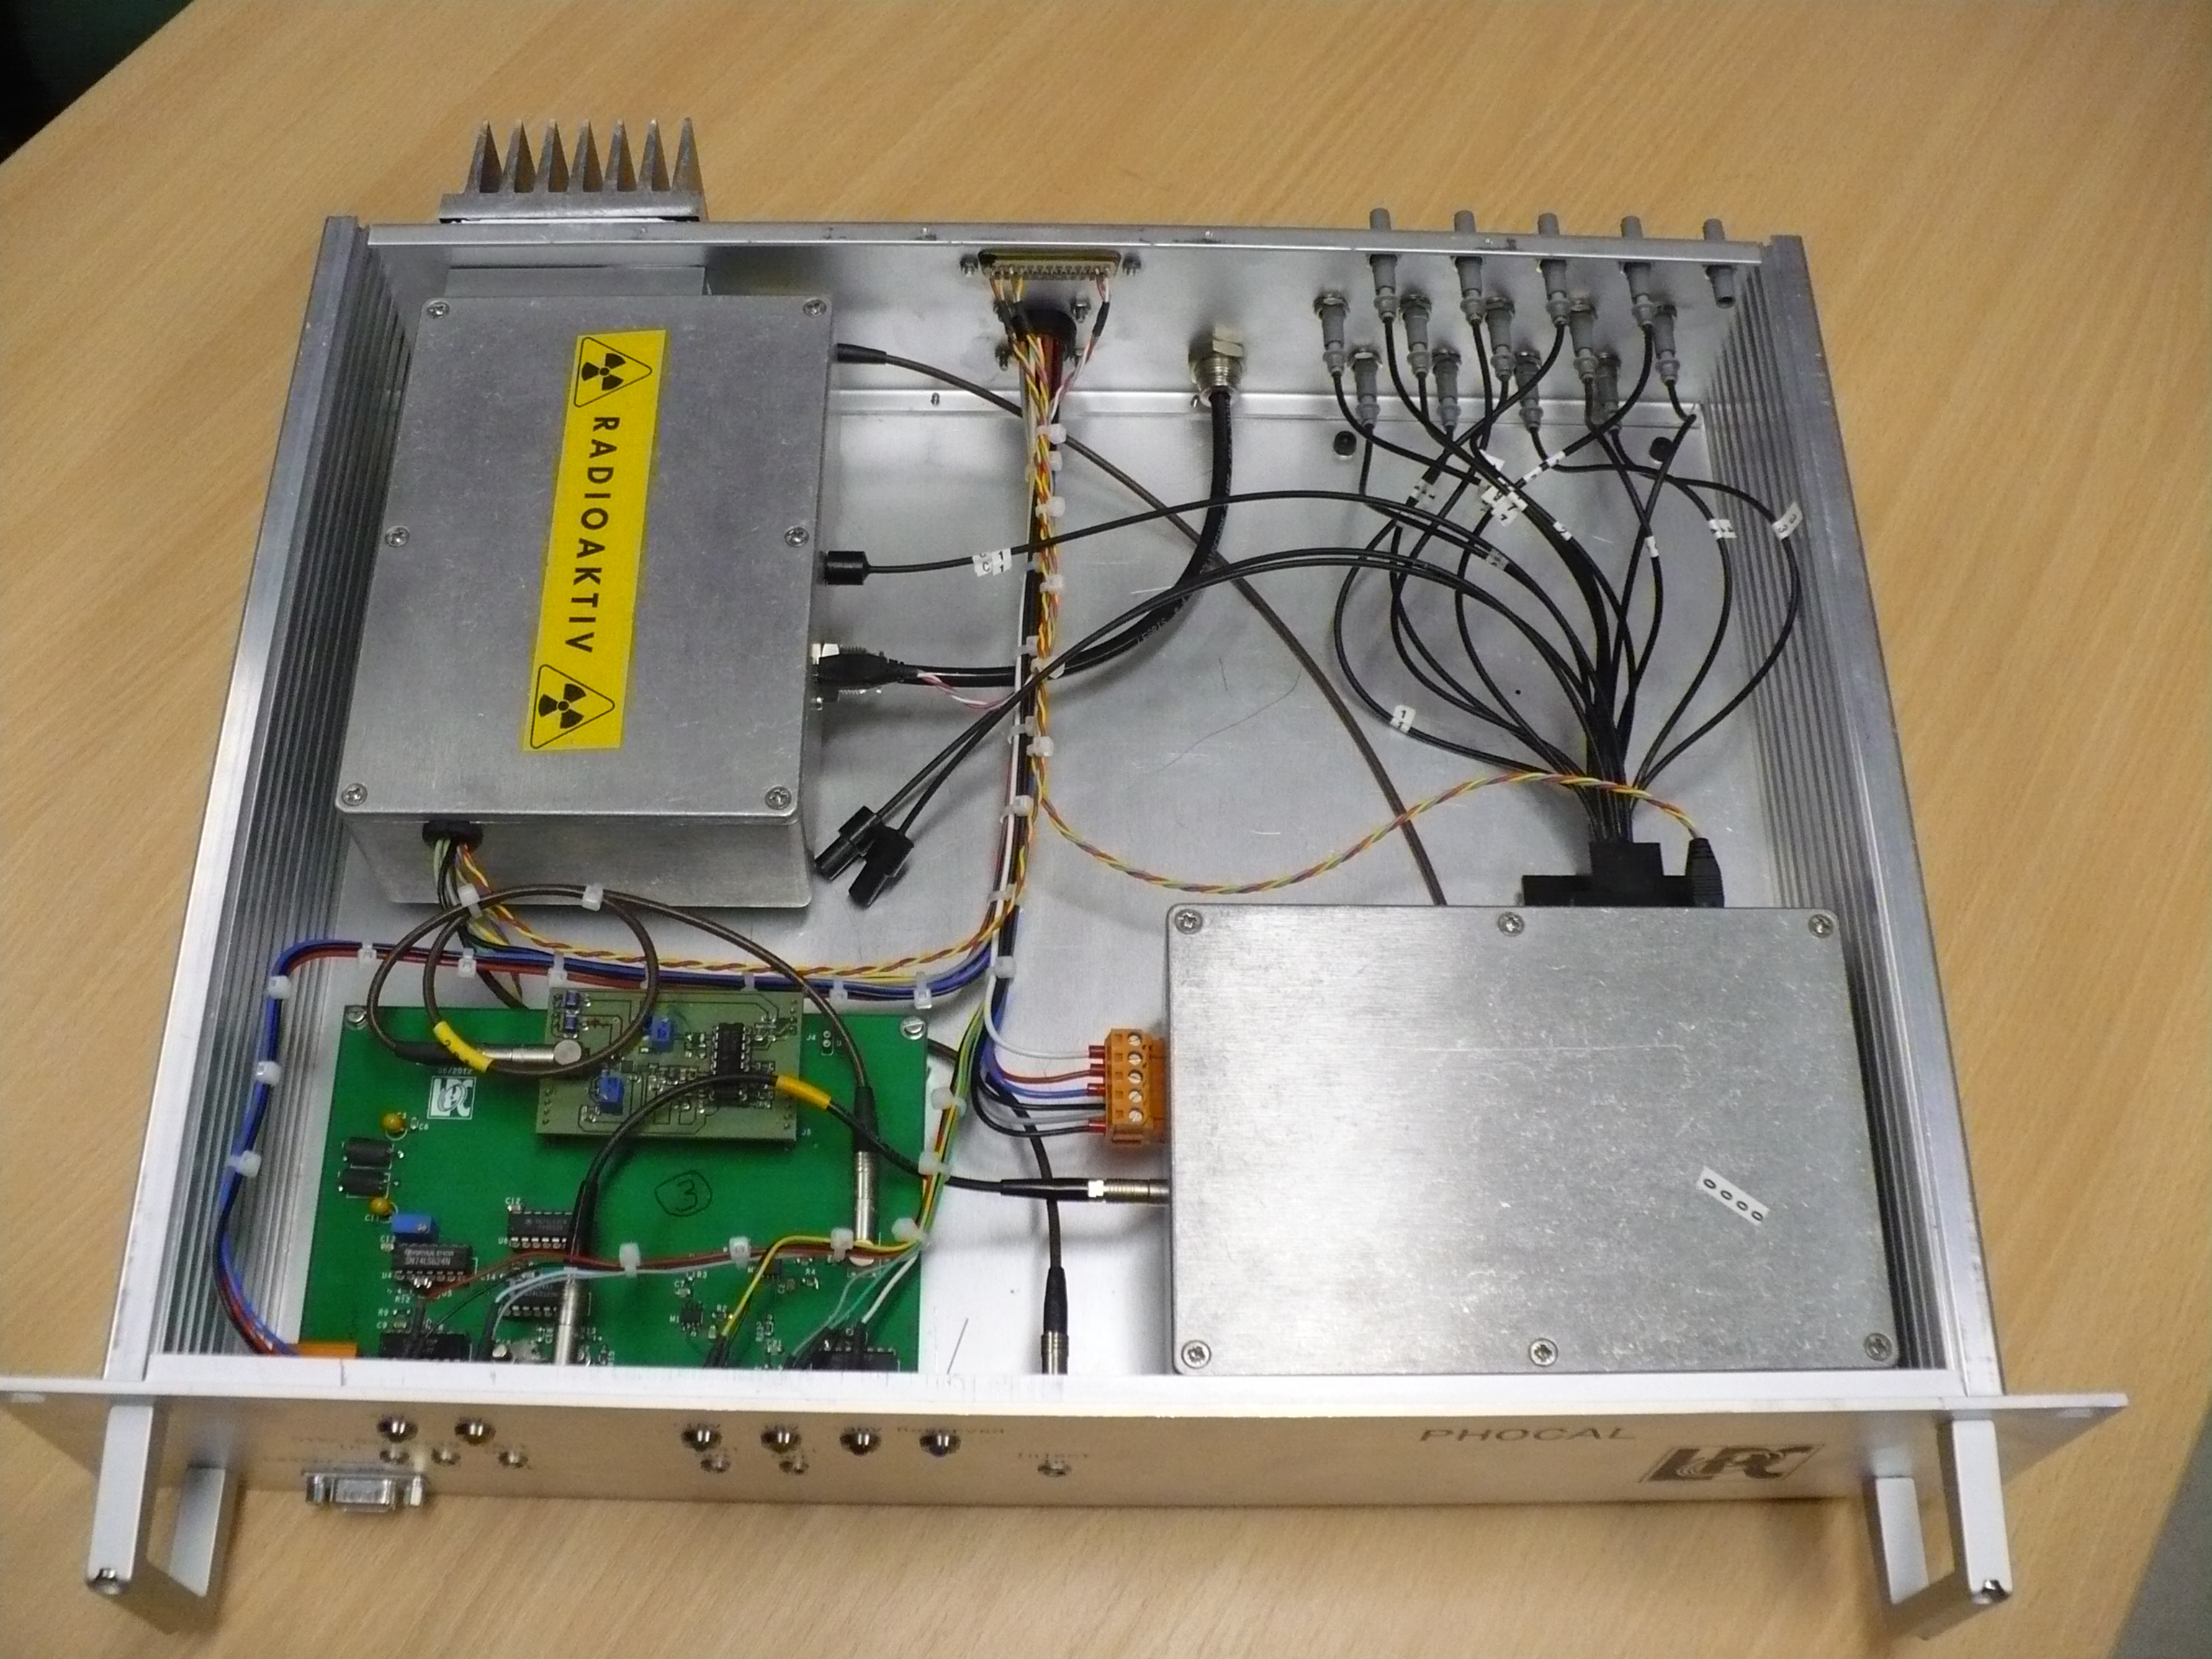
\includegraphics[height=6cm]{figures/phocal1.JPG}
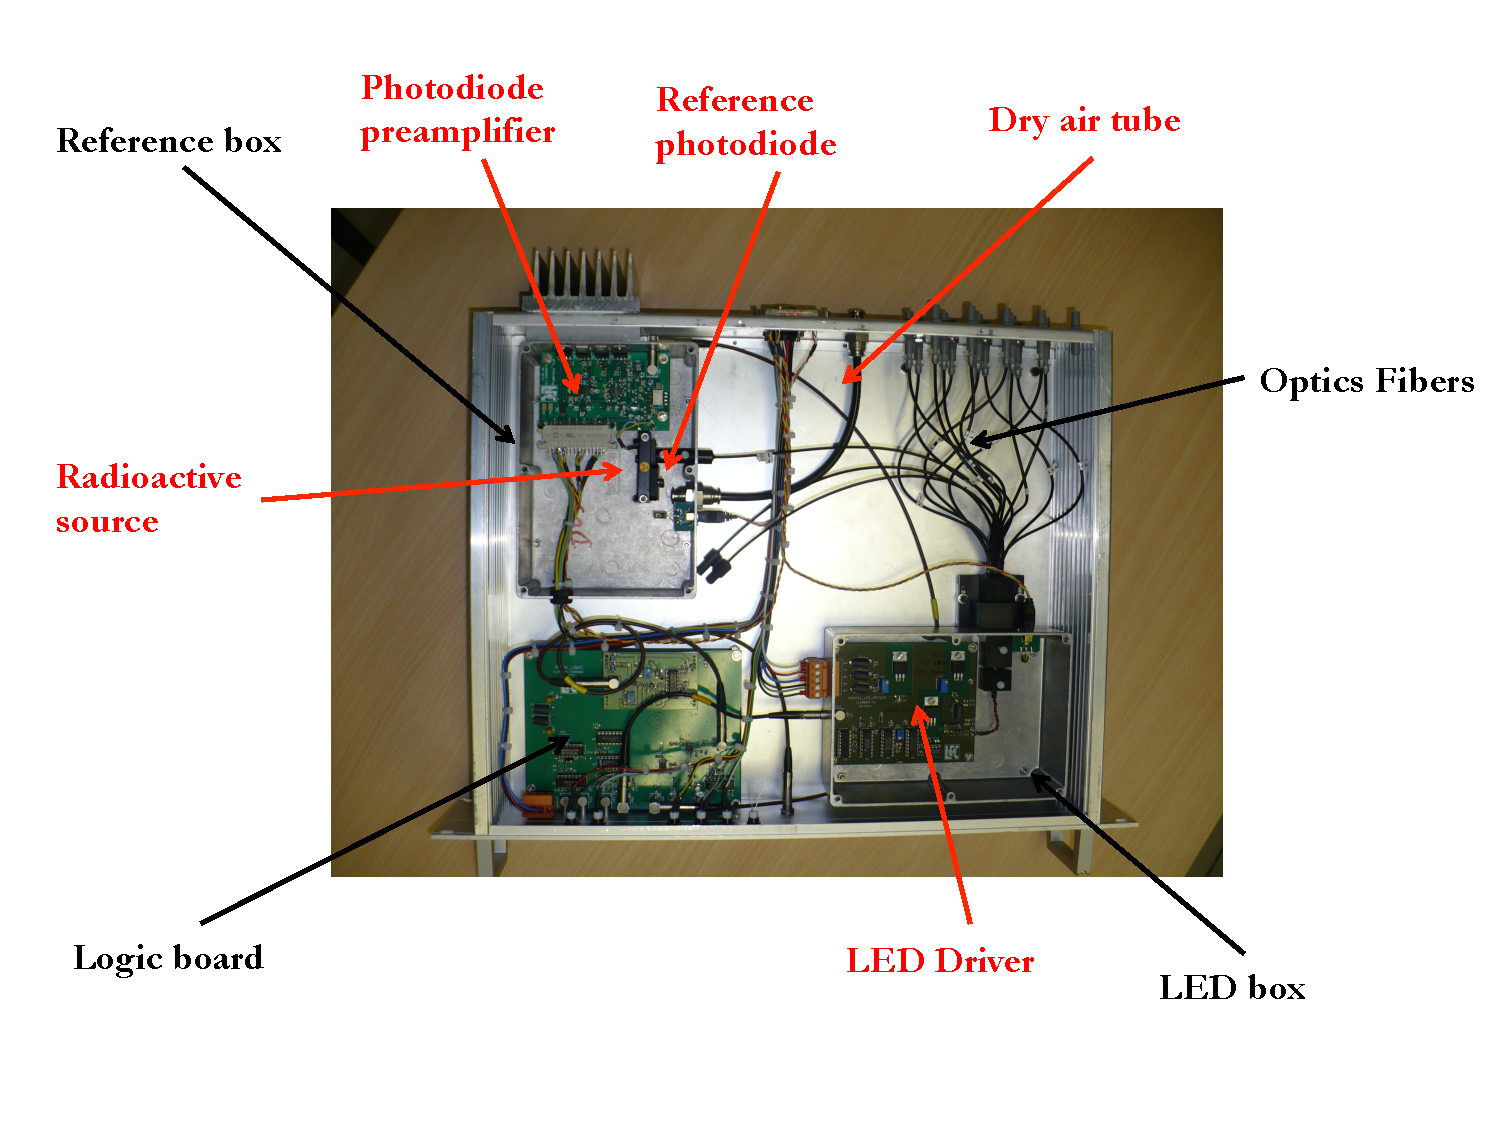
\includegraphics[height=10cm]{figures/phocal2_comm.pdf}
\caption{View of the PHOCAL system}\label{fig:lasphocal}
\end{figure}